\section{Overview}\label{sec:overview}

\begin{figure}
  \centering
  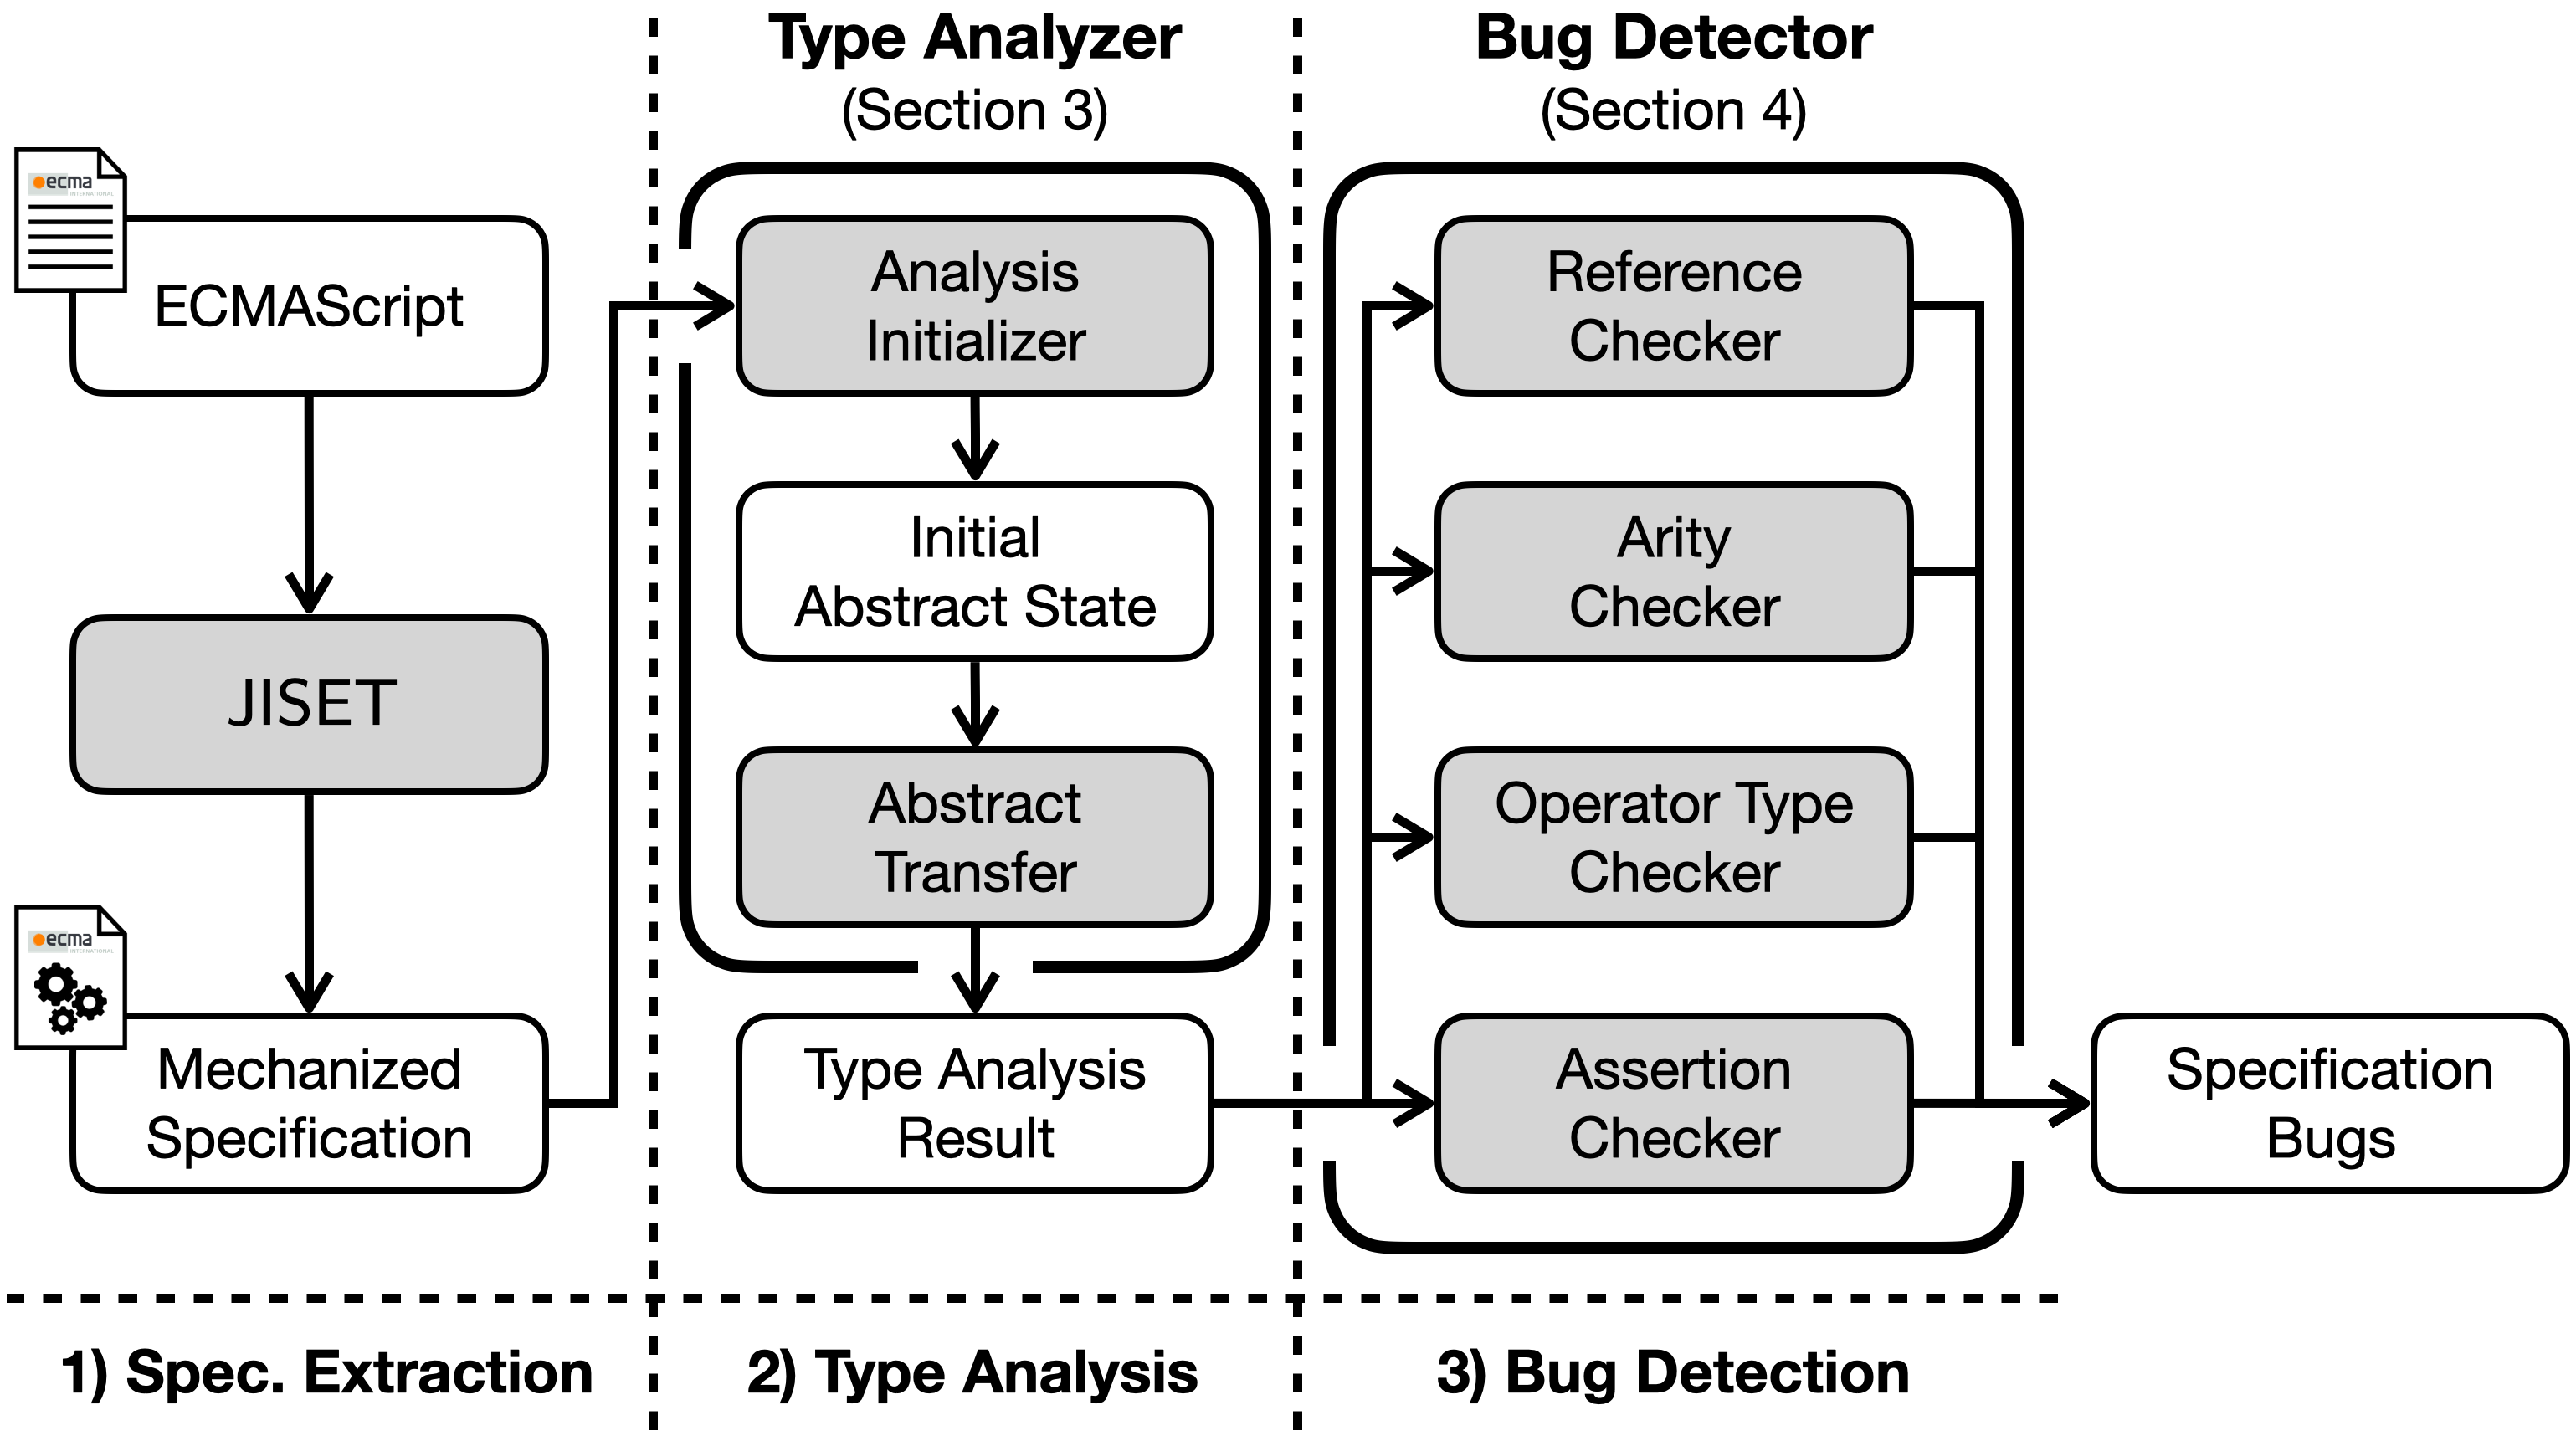
\includegraphics[width=0.48\textwidth]{img/overall}
  \vspace*{-1.5em}
  \caption{Overall structure of $\tool$: a type analyzer and a bug detector for
  mechanized specifications extracted from ECMAScript by $\jiset$.}
  \label{fig:overall}
\end{figure}

In this section, we demonstrate overall structure of $\tool$ depicted in
Figure~\ref{fig:overall} with a simple motivating example.

\begin{figure*}[t]
  \centering
  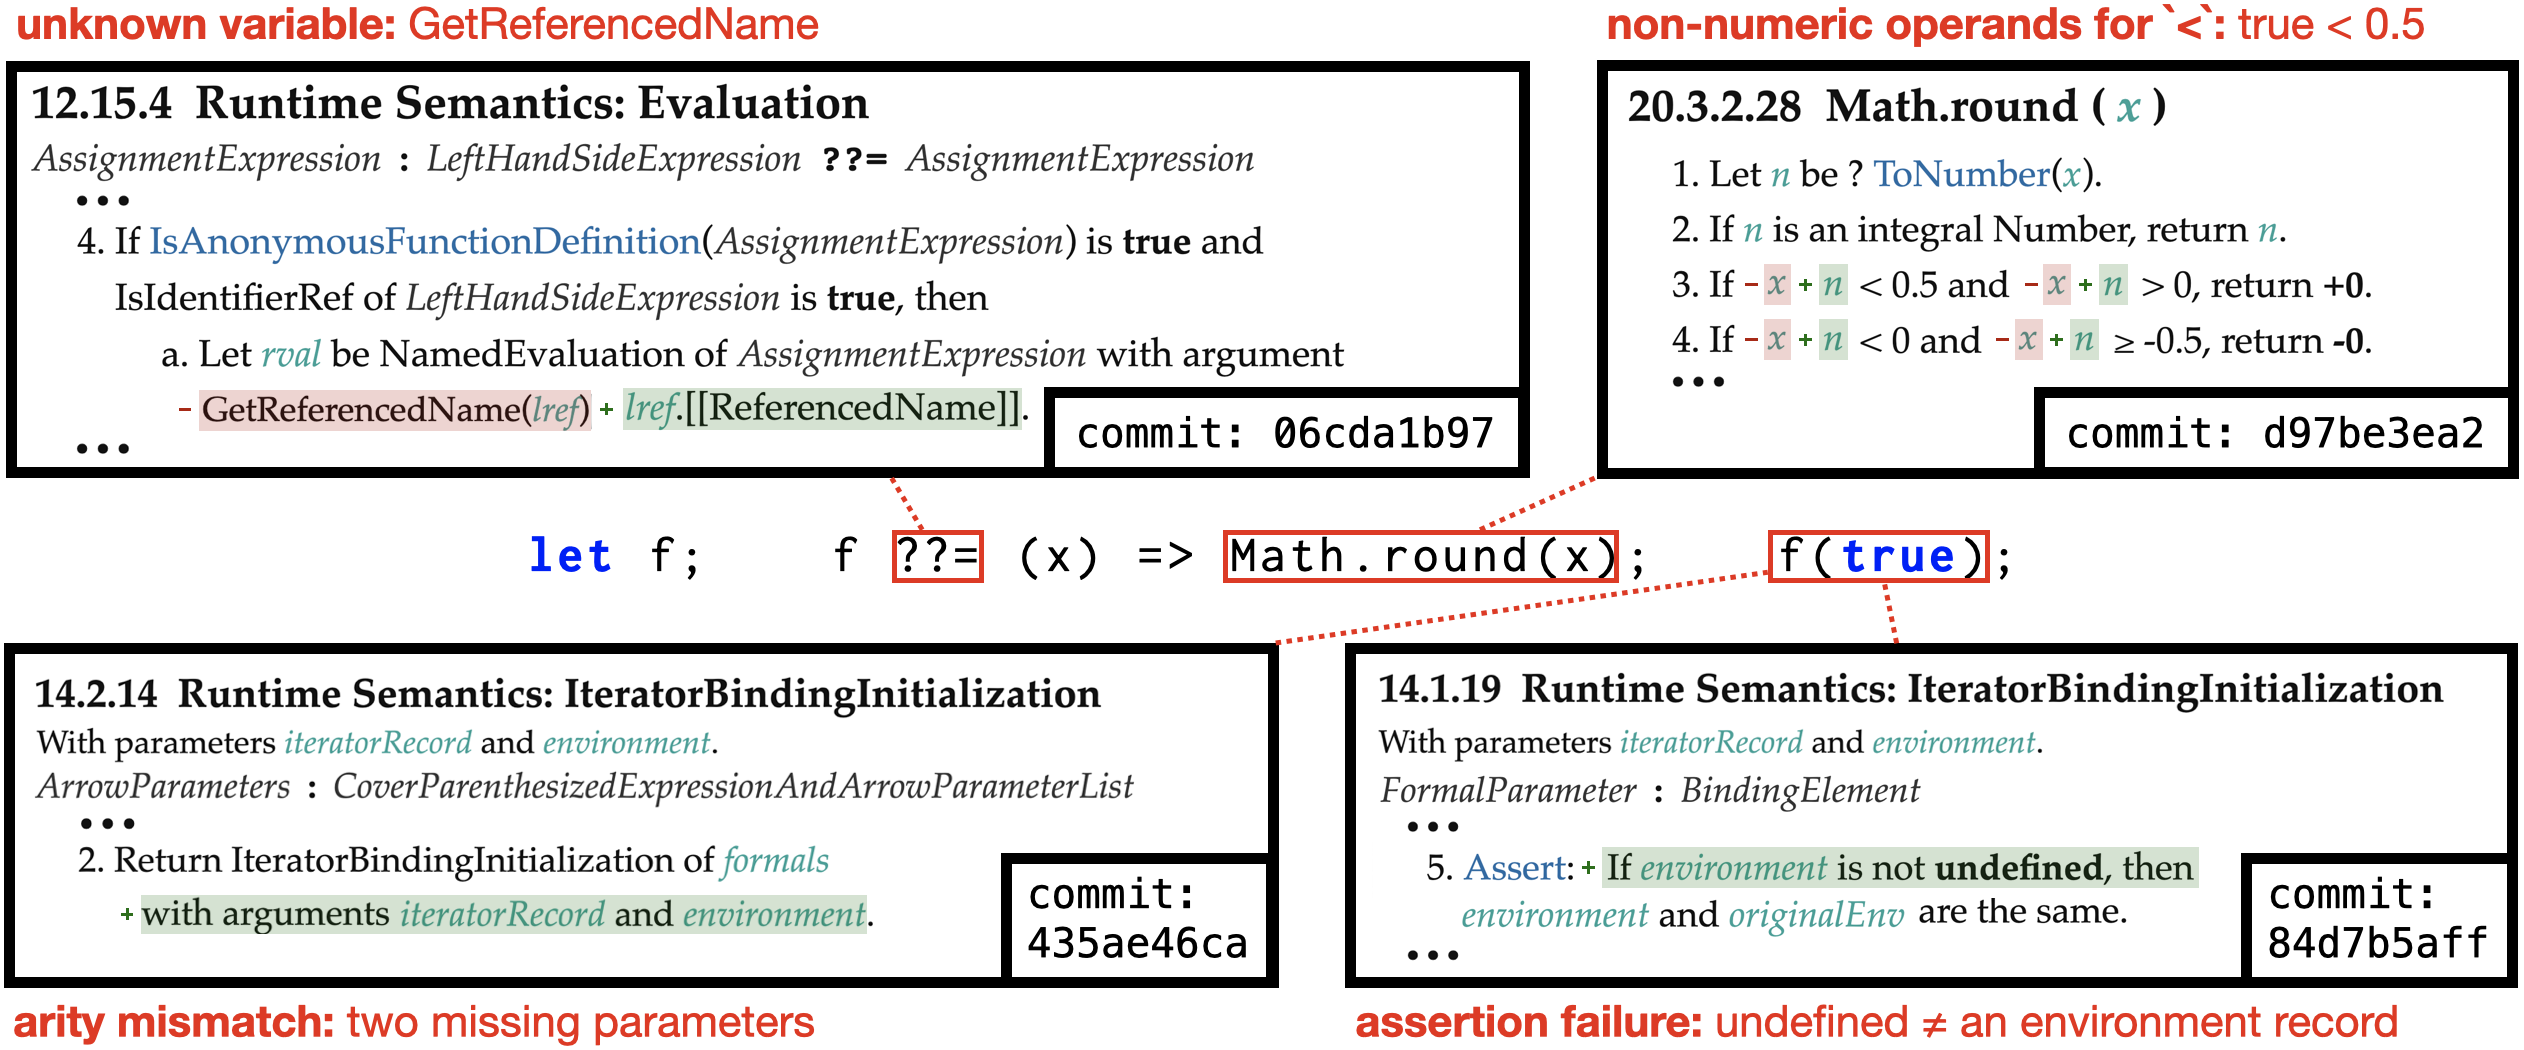
\includegraphics[width=0.85\textwidth]{img/example}
  \vspace*{-1em}
  \caption{A motivating example: a simple avaScript code with corresponding
  previous specification bugs and their bugfixs.}
  \label{fig:example}
\end{figure*}
